\documentclass{beamer}
\usepackage[utf8]{inputenc}
\usepackage{hyperref}
\usepackage{enumerate}
\usepackage{graphicx}
\usepackage{pgfplots}
\pgfplotsset{compat=1.16}
\graphicspath{{./images/}}
\usetheme{Warsaw}
\usecolortheme{whale}
\newcommand{\Aiden}{Aiden Taylor - B.Sc. in Computer Science}
\newcommand{\Noah}{Noah Pinel - B.Sc. in Computer Science}
\newcommand{\Ty}{Ty Irving - B.Sc. in Computer Science}
\setbeamertemplate{page number in head/foot}[framenumber]
%\setbeamertemplate{headline}{}

\begin{document}
\title[CPSC 530]{The Implementation and Comparison of the BCCBT Data Compression Algorithm}
\author[Group 17]{
\begin{tabular}{l}
    \Aiden \\ \Noah\\ \Ty\\ 
\end{tabular}}
\date{Apr. 11th, 2023}

\begingroup
    \setbeamertemplate{headline}{}
    \frame{\titlepage}
\endgroup

\begin{frame}
    \tableofcontents
\end{frame}

\section{Quiz Questions}
\begin{frame}
\begin{enumerate}[1.]
\item What specific type of Binary Tree is used in the implementation of the BCCBT Data Compression Algorithm?
Describe at least one discussed property of this type of Binary Tree.
\item Given the specific binary tree needed for the BCCBT algorithm, where the 
tree's nodes correspond to symbols in an arbitrary alphabet $\Sigma$.
Denote a symbol $\phi$, such that $\phi$ is in our arbitrary alphabet $\Sigma$.
Note, $\phi$ is \textbf{NOT} the root of the tree.\\
How is the bit code generated for the symbol $\phi$?
\item Does the BCCBT Data Compression Algorithm make use of the frequency/probability
of each unique symbol in the source file? Explain why or why not.
\end{enumerate}
\end{frame}


\section{Pseudocode}
\begin{frame}
\begin{center}
Bit Code Complete Binary Tree (BCCBT)
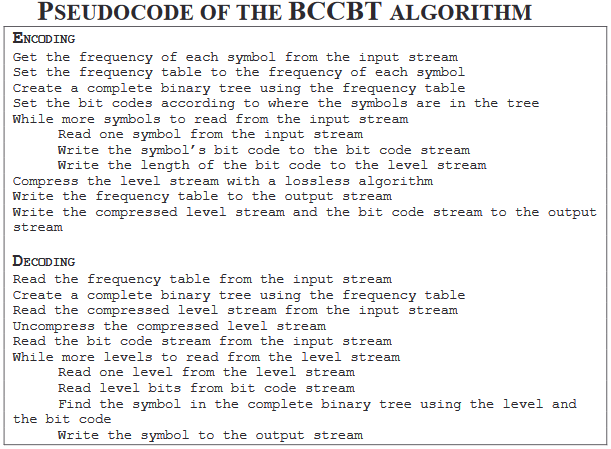
\includegraphics[scale=0.55]{pseudocode}
\end{center}
\end{frame}

\section{Example}
\begin{frame}
\begin{center}
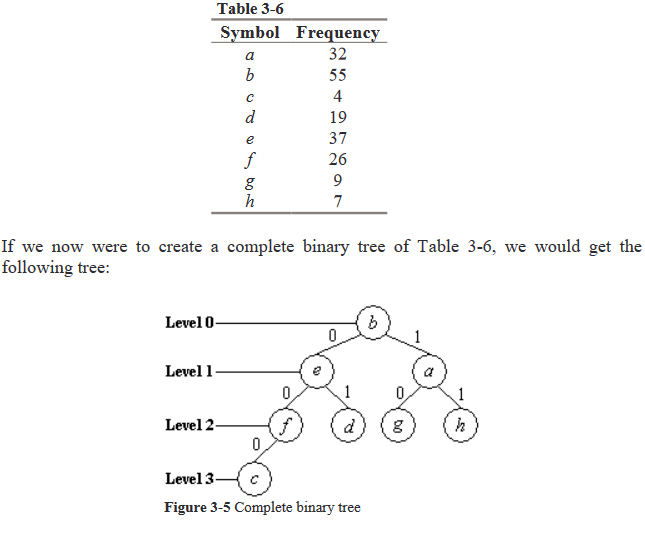
\includegraphics[scale=0.55]{example}
\end{center}
\end{frame}

\subsection{Complete Binary Trees and Frequencies}
\begin{frame}
Properties of Complete Binary Trees:
\begin{itemize}
\item All levels are completely full except possibly the lowest level.
\item Filled from left to right at each level. i.e. Tree leans left.
\item The number of nodes at level $n$ is $2^n$.
\end{itemize}
\end{frame}

\begin{frame}
\begin{center}
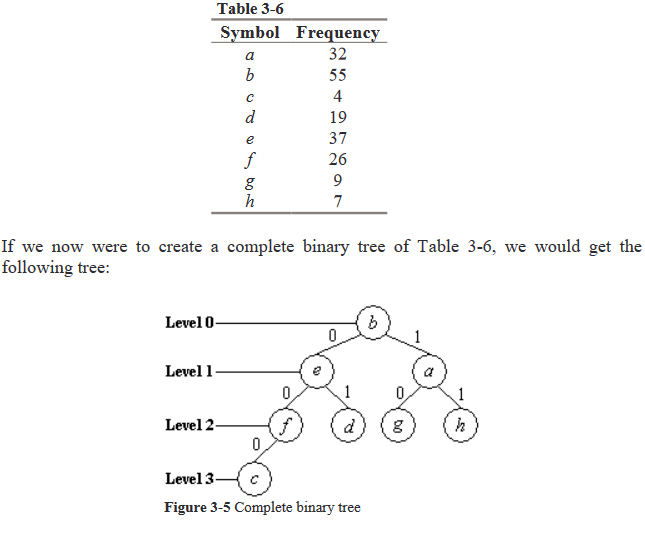
\includegraphics[scale=0.55]{example}
\end{center}
\end{frame}

\subsection{Encoding and Decoding}
\begin{frame}
    \frametitle{Step 1: Find the frequency Table}
    Given an alphabet $\Sigma =\{a, b, c, d, e, f, g, h\}$ where each symbol has the following frequency\\
    \begin{center}
        \begin{tabular}{ |c|c| } 
            \hline
            Symbol & Frequency \\ 
            \hline
            b & 55 \\
            e & 37 \\
            a & 32 \\ 
            f & 26 \\
            d & 19 \\
            g & 9 \\
            h & 7 \\ 
            c & 4 \\ 
            \hline
        \end{tabular}    
    \end{center}
\end{frame}

\begin{frame}
    \frametitle{Step 2: Generate Complete Tree and Get Bit Codes}

    \begin{center}
        \begin{minipage}{0.2\textwidth}
          \centering
          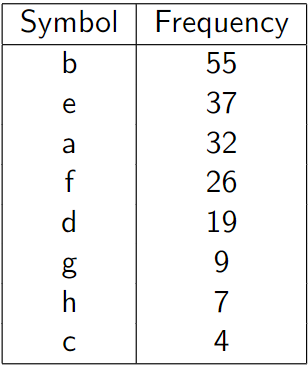
\includegraphics[scale=0.35]{images/freqtbl.png}
        \end{minipage}
        \hfill
        \begin{minipage}{0.6\textwidth}
          \centering
          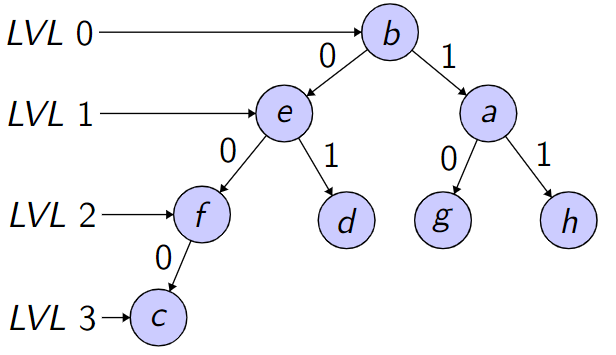
\includegraphics[scale=.35]{images/bintree.png}
        \end{minipage}
    \end{center}
    Wait, these bit codes are not uniquely decodable, how do we fix it?
    \begin{center}
        \begin{tabular}{|c|c|c|c|c|c|c|c|}
            \hline
            \multicolumn{8}{|c|}{BIT CODES} \\
            \hline
            a & b & c & d & e & f & g & h \\
            \hline
            1  & NULL  & 000  & 01  & 0  & 00  & 10  & 11\\
            \hline
        \end{tabular}
    \end{center}
\end{frame}

\begin{frame}
    \frametitle{Step 3:Making Uniquely Decodable Strings}
The solution, append the symbols level to its bit code. The bit strings are now uniquely decodable.\\
\large\textbf{Ex}) Say we want to encode the string `feed',
encoding would look like this: $[2]00[1]0[1]0[2]01$, where the number between the $[]$ 
specifies the level in the tree.
\begin{center}
    \begin{minipage}{0.2\textwidth}
      \centering
      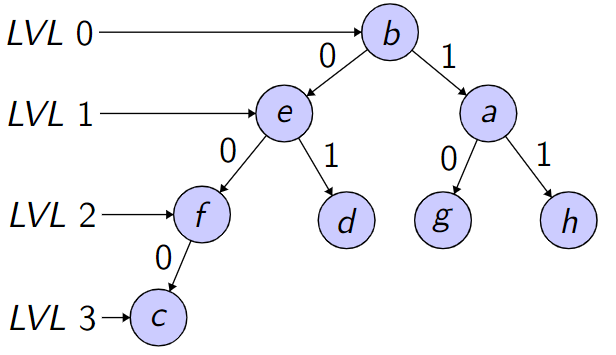
\includegraphics[scale=0.35]{images/bintree.png}
    \end{minipage}
    \hfill
    \begin{minipage}{0.4\textwidth}
      \centering
      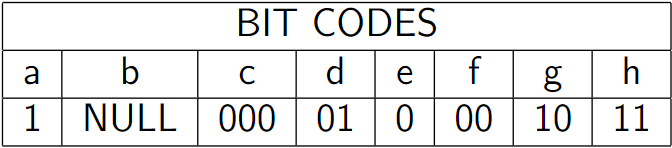
\includegraphics[scale=.29]{images/bitcode.png}
    \end{minipage}
\end{center}
\end{frame}

\begin{frame}
    \frametitle{Step 4: Decoding an Encrypted String}

    \begin{minipage}[t]{0.6\linewidth}
        Encrypted String: [1]0[2]01[2]10[1]0

        We first look at [1]. This is telling us the symbol is in LVL 1. The next bit, 0, tells us how we should walk the tree, in this case to the left once. We arrive at symbol e. Iterating through this n times:

        \begin{enumerate}
            \item $[1]0 \rightarrow$ e
            \item $[2]01 \rightarrow$ d
            \item $[2]10 \rightarrow$ g
            \item $[1]0 \rightarrow$ e
        \end{enumerate}

        $[1]0[2]01[2]10[1]0 \Rightarrow$ `edge' 
    \end{minipage}
    \hfill
    \begin{minipage}[t]{0.35\linewidth}
        \vspace{0pt}
        \begin{flushright}
            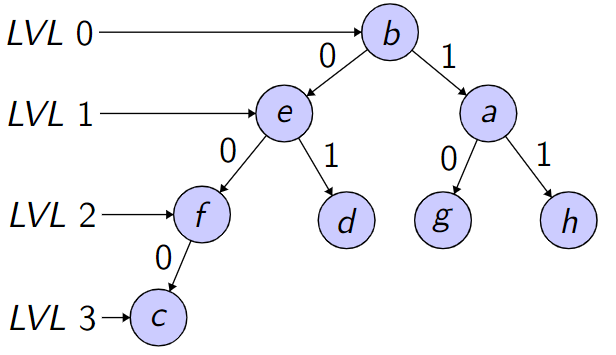
\includegraphics[scale=0.3]{images/bintree.png}
            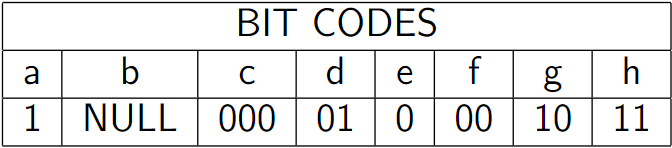
\includegraphics[scale=0.25]{images/bitcode.png}
        \end{flushright}
    \end{minipage}
\end{frame}


\section{Test Results}
\subsection{Factors}
\begin{frame}
Some factors we will be using to analyze and compare these algorithms are as follows:
\begin{enumerate}
    \item Compression Time 
    \item Decompression Time
    \item Saving Percentage = $\frac{Original\ File\ Size\ -\ Compressed\ File\ Size}{Original\ File\ Size}$
    \item Compression Ratio = $\frac{Compressed\ File\ Size}{Original\ File\ Size}$
\end{enumerate}
\end{frame}
\subsection{Test Result Graphs}
\begin{frame}
    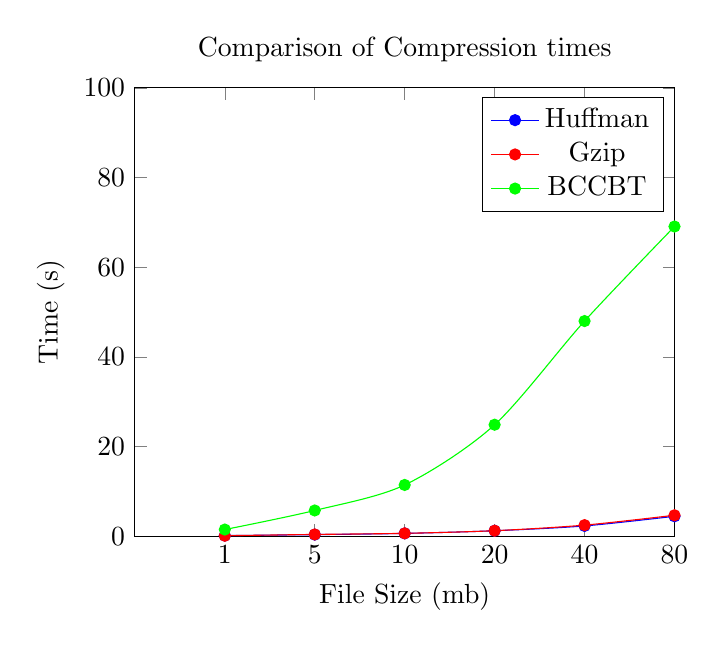
\begin{tikzpicture}
        \begin{axis}[
            xlabel=File Size (mb),
            ylabel=Time (s),
            xmin=0, xmax=6,
            ymin=0, ymax=100,
            xtick={1,2,3,4,5,6},
            xticklabels={1,5,10,20,40,80},   % <---
            ytick={0,20,...,100},
            title={Comparison of Compression times}
                    ]
        \addplot[smooth,mark=*,blue] plot coordinates {
            (1,0.129)(2,0.351)(3,0.625)(4,1.216)(5,2.293)(6,4.443)
        };
        \addlegendentry{Huffman}
        
        \addplot[smooth,color=red,mark=*]
            plot coordinates {
                (1,0.107)(2,0.394)(3,0.638)(4, 1.228)(5,2.472)(6, 4.671)
        
            };
        \addlegendentry{Gzip}
        \addplot[smooth,color=green,mark=*]
            plot coordinates {
                (1,1.485)(2,5.739)(3,11.430)(4,24.864)(5,47.988)(6, 69.076)
            };
        \addlegendentry{BCCBT}
        
        \end{axis}
    \end{tikzpicture}
\end{frame}

\begin{frame}
    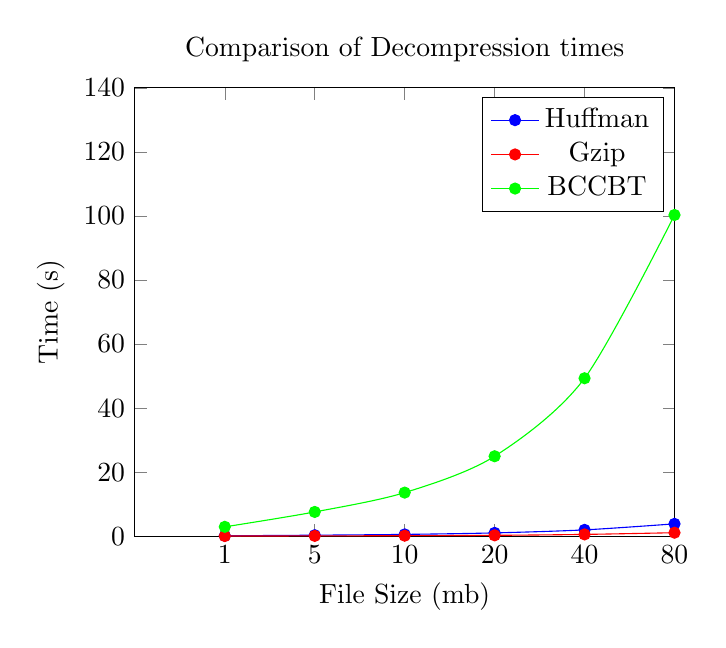
\begin{tikzpicture}
        \begin{axis}[
            xlabel=File Size (mb),
            ylabel=Time (s),
            xmin=0, xmax=6,
            ymin=0, ymax=140,
            xtick={1,2,3,4,5,6},
            xticklabels={1,5,10,20,40,80},   % <---
            ytick={0,20,...,140},
            title={Comparison of Decompression times}
                    ]
        \addplot[smooth,mark=*,blue] plot coordinates {
            (1,0.123)(2,0.313)(3,0.561)(4,1.030)(5,1.974)(6, 3.853)
        };
        \addlegendentry{Huffman}
        
        \addplot[smooth,color=red,mark=*]
            plot coordinates {
                (1,0.045)(2,0.092)(3,0.154)(4, 0.269)(5,0.557)(6, 1.091)
        
            };
        \addlegendentry{Gzip}
        \addplot[smooth,color=green,mark=*]
            plot coordinates {
                (1,2.92)(2,7.576)(3,13.611)(4,24.964)(5, 49.321)(6, 100.311)
            };
        \addlegendentry{BCCBT}
        
        \end{axis}
    \end{tikzpicture}
\end{frame}

\begin{frame}
    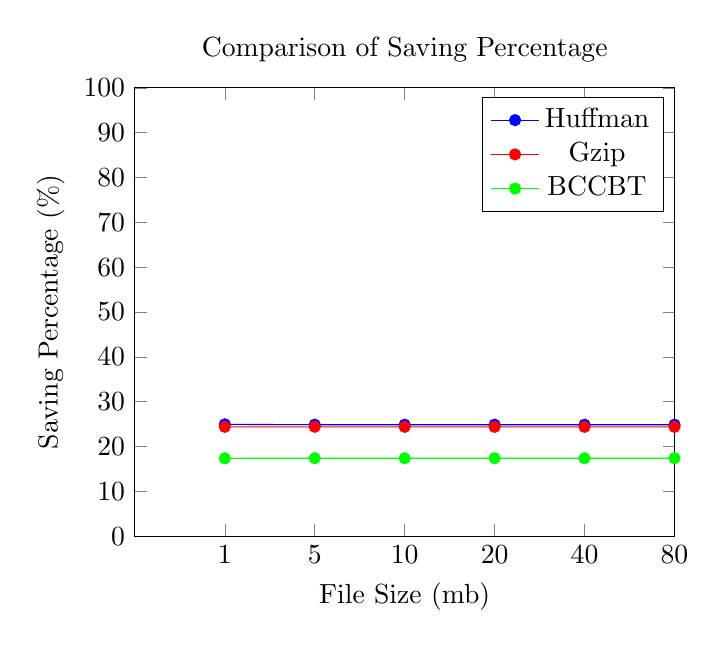
\begin{tikzpicture}
        \begin{axis}[
            xlabel=File Size (mb),
            ylabel=Saving Percentage (\%),
            xmin=0, xmax=6,
            ymin=0, ymax=100,
            xtick={1,2,3,4,5,6},
            xticklabels={1,5,10,20,40,80},   % <---
            ytick={0,10,...,100},
            title={Comparison of Saving Percentage}
                    ]
        \addplot[smooth,mark=*,blue] plot coordinates {
            (1,24.95)(2,24.87)(3,24.87)(4,24.87)(5,24.87)(6,24.87)
        };
        \addlegendentry{Huffman}
        
        \addplot[smooth,color=red,mark=*]
            plot coordinates {
                (1,24.39)(2,24.40)(3,24.39)(4,24.39)(5,24.39)(6,24.39)
            };
        \addlegendentry{Gzip}
        \addplot[smooth,color=green,mark=*]
            plot coordinates {
                (1,17.37)(2,17.39)(3,17.38)(4,17.39)(5,17.39)(6,17.39)
            };
        \addlegendentry{BCCBT}
        
        \end{axis}
    \end{tikzpicture}
\end{frame}


\definecolor{mybabyblue}{RGB}{140,216,231}
\definecolor{mysoftgreen}{RGB}{120,233,212}
\begin{frame}
    \begin{tikzpicture}
        \begin{axis}[
            title={BCCBT Compression Sizes},
            xlabel={File size (MB)},
            ylabel={Size after compression (MB)},
            ymin=0, ymax=120,
            ytick={0,20,40,60,80,100,120},
            xtick={1,2,3,4,5,6},
            xticklabels={1,5, 10, 20, 40, 80},
            ybar=5pt,
            bar width=10pt,
        ]
        
        \addplot[
            fill=mybabyblue,
            ]
            coordinates {
            (1,1)(2,5)(3,10)(4,20)(5,40)(6,80)
            };
            \addlegendentry{Initial file size}
            
        \addplot[
            fill=mysoftgreen,
            ]
            coordinates {
            (1,0.8)(2,4.17)(3,8.6)(4,16.6)(5,33.3)(6,66.7)
            };
            \addlegendentry{Compressed file size}
        \end{axis}
        \end{tikzpicture}
\end{frame}
\begin{frame}
    \begin{tikzpicture}
        \begin{axis}[
            title={Gzip Compression Sizes},
            xlabel={File size (MB)},
            ylabel={Size after compression (MB)},
            ymin=0, ymax=120,
            ytick={0,20,40,60,80,100,120},
            xtick={1,2,3,4,5,6},
            xticklabels={1,5, 10, 20, 40, 80},
            ybar=5pt,
            bar width=10pt,
        ]
        
        \addplot[
            fill=mybabyblue,
            ]
            coordinates {
            (1,1)(2,5)(3,10)(4,20)(5,40)(6,80)
            };
            \addlegendentry{Initial file size}
            
        \addplot[
            fill=mysoftgreen,
            ]
            coordinates {
            (1,0.76)(2,3.8)(3,7.6)(4,15.2)(5,30.5)(6,59)
            };
            \addlegendentry{Compressed file size}
        \end{axis}
        \end{tikzpicture}
\end{frame}

\begin{frame}
    \begin{tikzpicture}
        \begin{axis}[
            title={Huffman Compression Sizes},
            xlabel={File size (MB)},
            ylabel={Size after compression (MB)},
            ymin=0, ymax=120,
            ytick={0,20,40,60,80,100,120},
            xtick={1,2,3,4,5,6},
            xticklabels={1,5, 10, 20, 40, 80},
            ybar=5pt,
            bar width=10pt,
        ]
        
        \addplot[
            fill=mybabyblue,
            ]
            coordinates {
            (1,1)(2,5)(3,10)(4,20)(5,40)(6,80)
            };
            \addlegendentry{Initial file size}
            
        \addplot[
            fill=mysoftgreen,
            ]
            coordinates {
            (1,0.758)(2,3.79)(3,7.58)(4,15.17)(5,30.35)(6,60.7)
            };
            \addlegendentry{Compressed file size}
        \end{axis}
        \end{tikzpicture}
\end{frame}
\subsection{Summary}
\begin{frame}
    \frametitle{Result Summary}
    Huffman and GZip both performed better than the BCCBT algorithm especially during 
    compression and decompression times.  The main factor behind this run time for the 
    compression and decompression time is how it was implemented in our code with traversing
    the tree, this algorithm also requires a lot of memory space for large files.
    \begin{itemize}
        \item{BCCBT was slightly behind GZip and Huffman for saving percentages however
        the gap between them did not grow.}
        \item{BCCBT fell behind heavily in compression and decompression times as files
        sizes got larger.}
    \end{itemize}
\end{frame}

\section{Conclusion}
\begin{frame}
 Ty should probably add a slide to wrap up what he just talked about, before we say we are done 
 rn the transition does not look natural
\end{frame}

\section{Q\&A}
\begin{frame}
Thank you for listening! Any questions?
\end{frame}

\end{document}
% CODE FOR TREE GEN
% \begin{tikzpicture}[scale=0.1]
%     \tikzstyle{every node}+=[inner sep=0pt]
%     \draw [fill=blue!20] (48.4,-25.1) circle (3);
%     \draw (48.4,-25.1) node {$a$};
%     \draw [fill=blue!20] (38,-16.5) circle (3);
%     \draw (38,-16.5) node {$b$};
%     \draw [fill=blue!20] (13.5,-46.7) circle (3);
%     \draw (13.5,-46.7) node {$c$};
%     \draw [fill=blue!20] (33.4,-36.4) circle (3);
%     \draw (33.4,-36.4) node {$d$};
%     \draw [fill=blue!20] (26.8,-25.1) circle (3);
%     \draw (26.8,-25.1) node {$e$};
%     \draw [fill=blue!20] (18.1,-35.8) circle (3);
%     \draw (18.1,-35.8) node {$f$};
%     \draw [fill=blue!20] (43.6,-36.4) circle (3);
%     \draw (43.6,-36.4) node {$g$};
%     \draw [fill=blue!20] (56.9,-36.4) circle (3);
%     \draw (56.9,-36.4) node {$h$};
%     \draw [black] (35.62,-18.33) -- (29.18,-23.27);
%     \fill [black] (29.18,-23.27) -- (30.12,-23.18) -- (29.51,-22.39);
%     \draw (31.39,-20.3) node [above] {$0$};
%     \draw [black] (40.31,-18.41) -- (46.09,-23.19);
%     \fill [black] (46.09,-23.19) -- (45.79,-22.29) -- (45.15,-23.06);
%     \draw (44.21,-20.31) node [above] {$1$};
%     \draw [black] (50.2,-27.5) -- (55.1,-34);
%     \fill [black] (55.1,-34) -- (55.02,-33.06) -- (54.22,-33.66);
%     \draw (53.23,-29.35) node [right] {$1$};
%     \draw [black] (47.23,-27.86) -- (44.77,-33.64);
%     \fill [black] (44.77,-33.64) -- (45.55,-33.1) -- (44.63,-32.71);
%     \draw (45.26,-29.8) node [left] {$0$};
%     \draw [black] (24.91,-27.43) -- (19.99,-33.47);
%     \fill [black] (19.99,-33.47) -- (20.89,-33.17) -- (20.11,-32.54);
%     \draw (21.89,-29.02) node [left] {$0$};
%     \draw [black] (16.93,-38.56) -- (14.67,-43.94);
%     \fill [black] (14.67,-43.94) -- (15.44,-43.39) -- (14.52,-43);
%     \draw (15.06,-40.31) node [left] {$0$};
%     \draw [black] (28.31,-27.69) -- (31.89,-33.81);
%     \fill [black] (31.89,-33.81) -- (31.92,-32.87) -- (31.05,-33.37);
%     \draw (30.75,-29.51) node [right] {$1$};
%     \draw [black] (7.2,-16.5) -- (35,-16.5);
%     \draw (6.7,-16.5) node [left] {$LVL\mbox{ }0$};
%     \fill [black] (35,-16.5) -- (34.2,-16) -- (34.2,-17);
%     \draw [black] (7.3,-25.1) -- (23.8,-25.1);
%     \draw (6.8,-25.1) node [left] {$LVL\mbox{ }1$};
%     \fill [black] (23.8,-25.1) -- (23,-24.6) -- (23,-25.6);
%     \draw [black] (7.5,-35.8) -- (15.1,-35.8);
%     \draw (7,-35.8) node [left] {$LVL\mbox{ }2$};
%     \fill [black] (15.1,-35.8) -- (14.3,-35.3) -- (14.3,-36.3);
%     \draw [black] (7.5,-46.7) -- (10.5,-46.7);
%     \draw (7,-46.7) node [left] {$LVL\mbox{ }3$};
%     \fill [black] (10.5,-46.7) -- (9.7,-46.2) -- (9.7,-47.2);
%     \end{tikzpicture}
% \end{center}